\begin{frame}
  \frametitle{Kerr effect: Mathematical formulation}

  With a centrosymmetric and isotropic medium the important term is
  \[
  \mathbf P = \epsilon_0 ( \chi\order1 \mathbf E +
  {\chi\order2 \mathbf E^2} + \textcolor{red}{\chi\order3 \mathbf E^3} \dots )
  \]
\end{frame}

\begin{frame}
  \frametitle{Suspectibility}

  The refractive index of the medium will then be intensity dependent. 
  \begin{align*}
    n &= \sqrt{1 + \chi_1 + \chi_3 |\mathcal{E}|^2}\\
    &\simeq n_0 + \tfrac{1}{2} n_2 |\mathcal{E}|^2,
  \end{align*}
\end{frame}

\begin{frame}
  \frametitle{Gaussion beams}
  Assume: Beam has a gaussian shape

  $\Rightarrow$ Refractive index is peaked at center.
  {\centering
  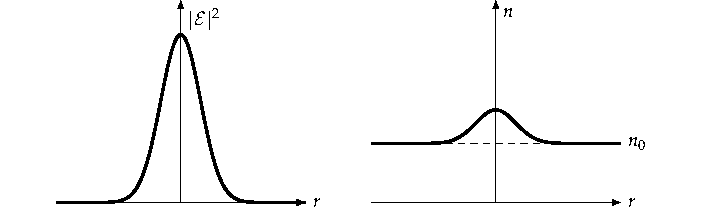
\includegraphics[width=1\columnwidth]{gaussrefrac}}

This is effectively a positive lens that will focus the beam. 
\end{frame}




%%% Local Variables: 
%%% mode: latex
%%% TeX-master: "nonlinearslides"
%%% End: 
